\documentclass[tikz, border=3mm]{standalone}
\usepackage{tikz}
\usetikzlibrary{shapes.geometric, arrows, positioning, fit, calc}
\usepackage{fontspec}
\setmainfont{Times New Roman}
\begin{document}
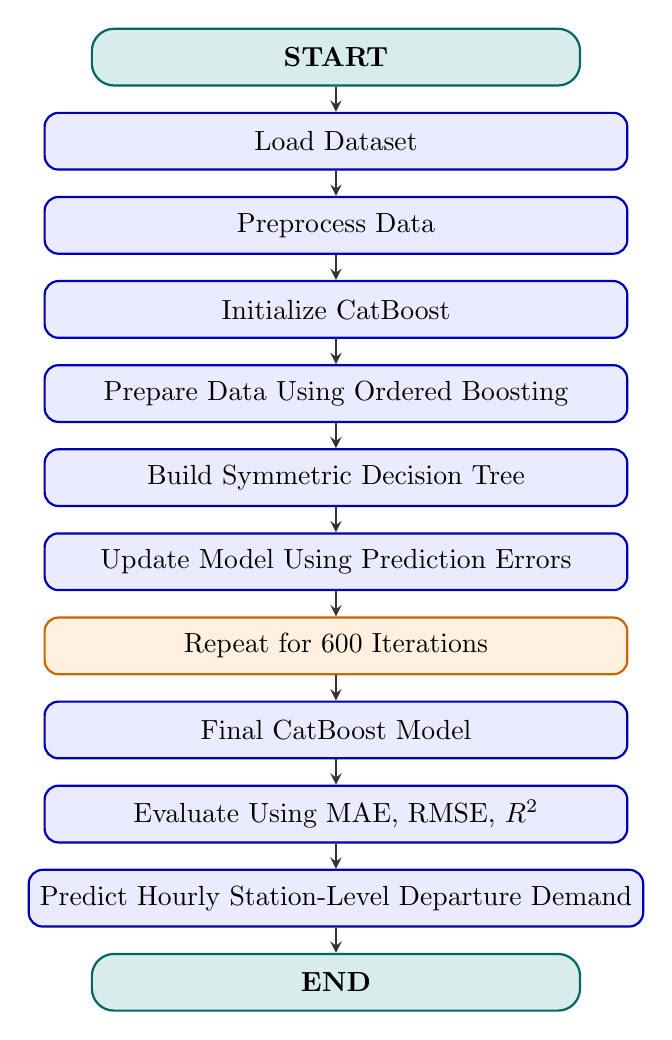
\begin{tikzpicture}[
    node distance=0.32cm,
    startstop/.style={rectangle, rounded corners=8pt, minimum width=6.2cm, minimum height=0.72cm, align=center, draw=teal!80!black, thick, fill=teal!15, font=\rmfamily\bfseries\normalsize, inner sep=4pt},
    proc/.style={rectangle, rounded corners=5pt, minimum width=7.4cm, minimum height=0.72cm, align=center, draw=blue!70!black, thick, fill=blue!8, font=\rmfamily\normalsize, inner sep=4pt},
    boost/.style={rectangle, rounded corners=5pt, minimum width=7.4cm, minimum height=0.72cm, align=center, draw=orange!80!black, thick, fill=orange!12, font=\rmfamily\normalsize, inner sep=4pt},
    arrow/.style={thick, ->, >=stealth, draw=black!80}
]

\node (start) [startstop] {START};
\node (load) [proc, below=0.32cm of start] {Load Dataset};
\node (prep) [proc, below=0.32cm of load] {Preprocess Data};
\node (init) [proc, below=0.32cm of prep] {Initialize CatBoost};
\node (ord) [proc, below=0.32cm of init] {Prepare Data Using Ordered Boosting};
\node (tree) [proc, below=0.32cm of ord] {Build Symmetric Decision Tree};
\node (update) [proc, below=0.32cm of tree] {Update Model Using Prediction Errors};
\node (repeat) [boost, below=0.32cm of update] {Repeat for 600 Iterations};
\node (final) [proc, below=0.32cm of repeat] {Final CatBoost Model};
\node (eval) [proc, below=0.32cm of final] {Evaluate Using MAE, RMSE, $R^2$};
\node (predict) [proc, below=0.32cm of eval] {Predict Hourly Station-Level Departure Demand};
\node (end) [startstop, below=0.32cm of predict] {END};

\draw [arrow] (start) -- (load);
\draw [arrow] (load) -- (prep);
\draw [arrow] (prep) -- (init);
\draw [arrow] (init) -- (ord);
\draw [arrow] (ord) -- (tree);
\draw [arrow] (tree) -- (update);
\draw [arrow] (update) -- (repeat);
\draw [arrow] (repeat) -- (final);
\draw [arrow] (final) -- (eval);
\draw [arrow] (eval) -- (predict);
\draw [arrow] (predict) -- (end);

\end{tikzpicture}
\end{document}
